\chapter{Introducere}

\acrlong{iot} este unul din subiectele de cel mai mare interes în sfera tehnologiei,
alături de inteligența artificială, tehnologia blockchain și realitatea virtuală. 
Definiția exactă a acestui termen variază semnificativ atât în lucrările
științifice cât și în presă sau publicațiile companiilor din domeniul tehnologiei informației sau domenii adiacente. Prima dată utilizat de Kevin Ashton într-o prezentare ținută pentru Procter \& Gamble în anul 1999 (fapt amintit în articolul aceluiași autor, anume \citetitle{ashton_2009}), acesta se referea la dispozitivele care cu ajutorul senzorilor dau capacitatea computerelor de a "vedea", "auzi" și "simți" mediul înconjurător. Astăzi, atunci când vorbim de \acrshort{iot} înglobăm o gamă largă de concepte și dispozitive: rețele wireless, electrocasnice inteligente, automatizări rezidențiale sau industriale, vehicule autonome, toate se pot încadra sub eticheta \acrshort{iot}.

Probabil cea mai răspândită și populară aplicare a sistemelor \acrshort{iot} sunt locuințele inteligente. Datorită interesului crescut pentru eficientizarea consumului de energie, reducerea emisiilor de carbon, dar și al beneficiilor promise pentru calitatea vieții, locuințele și orașele inteligente interconectate folosind internetul au devenit un vis tehnologic atât al cetățenilor cât și al companiilor sau guvernelor. De la iluminare cu senzori de mișcare până la asistenți virtuali care ne învață preferințele legate de muzică sau temperatură, suntem tot mai înconjurați de \textit{lucruri} (\textit{things}) inteligente, interconectate, ce procesează cantități enorme de date despre mediul nostru, dar și despre noi. 

Deși este o nișă relativ tânără, rețelele de dispozitive inteligente își fac loc în tot mai multe industrii și domenii de activitate cu o lungă istorie. În fabricile moderne se utilizează rețele complexe de senzori, roboți și dispozitive de coordonare pentru a facilita linii de producție. În agricultură atât monitorizarea cât și îngrijirea culturilor se poate realiza folosind senzori și drone conectate la internet. În sectorul public există inițiative de digitalizare a infrastructurii și comunicării dintre instituții și cetățeni, scopul final fiind crearea de orașe cu adevărat inteligente. 

Pentru a asigura reușita implementării acestor noi tehnologii, considerăm că existența unor metodologii, tehnici și unelte de testare adaptate la complexitatea și provocările specifice sistemelor \acrshort{iot} este absolut necesară. Astfel, prezenta lucrare își propune să facă cunoscute cititorului principalele provocări întâlnite în testarea sistemelor \acrshort{iot}, ilustrând avantajele și dezavantajele mai multor metodologii întâlnite în literatura de specialitate sau industrie prin experimente practice. Aspectul de care vom fi cel mai preocupați este testarea securității.

În acest capitol va fi expusă detaliat motivația pentru alegerea temei lucrării și vom argumenta pe scurt relevanța acesteia, apoi vom continua prin parcurgerea unui scurt istoric al domeniului tratat, iar în final va fi prezentată structura capitolelor ce urmează.

\section{Motivația pentru temă}

M-am alăturat echipei de cercetare a proiectului \textit{\acrfull{sasha}} realizat de Universitatea din București în colaborare cu Universitatea Politehnică din București, motivat fiind de provocarea de a explora securitatea sistemelor informatice într-o arie relativ tânără a tehnologiei, în care lipsesc practicile consacrate. Am avut astfel oportunitatea de a înțelege provocările și obstacolele întâlnite în dezvoltarea aplicațiilor \acrshort{iot}, în particular a celor pentru locuințe inteligente, de a explora și analiza soluțiile și practicile existente, iar mai apoi am putut contribui la realizarea unui articol de cercetare alături de domnul profesor Ciprian Păduraru și doctorandul Rareș Cristea, anume \textbf{Building blocks for IoT testing - a benchmark of IoT apps and a functional testing framework} prezentat la \textbf{4th International Workshop on Software Engineering Research \& Practices for the Internet of Things (SERP4IoT 2022)}, articol care țintește să îmbunătățească metodele de evaluare și comparare al tehnicilor de testare din domeniul \acrlong{iot}, făcând primii pași spre construirea unui set de aplicații \acrshort{iot} destinate \textit{benchmarking}-ului.

Pentru a fructifica experiența acumulată în timpul activității mele de cercetare, am decis să realizez o lucrare despre contribuția în cadrul proiectului \acrshort{sasha} și pentru realizarea articolului științific menționat anterior. Am dorit de asemenea să validez relevanța setului de aplicații propus în articol prin realizarea de experimente de comparare a câtorva tehnici de testare regăsite în literatură și industrie, o atenție sporită fiind acordată tehnicilor de testare a securității.

\section{Scurt istoric al Internet of Things}

Conceptul de dispozitive interconectate există încă din timpul apariției telegrafului, însă primele inițiative cu adevărat moderne le întâlnim abia în anii 1980 - 1990. Prima discuție cu urmări practice despre dispozitive inteligente conectate într-o rețea apare în 1982, când studenții de la  Carnegie Mellon University au folosit un tonomat Coca-Cola modificat conectat la \textit{ARPANET} (precursorul internetului modern) pentru a raporta automat inventarul și încasările. În decursul a puțini ani, lucrări precum \citet{Weiser1999}, dar și alte publicații de presă sau academice au conturat viziunea despre dispozitivele interconectate și interacțiunea lor cu viețile noastre. \citet{Raji1994} descrie în abstractul lucrării sale rețelele inteligente astfel (tradus din engleză):

% Control networks move small packets of data to a large set of nodes, so as to integrate and automate everything from home appliances to entire factories

\say{Rețelele de control transportă pachete mici de date la un număr mare de noduri, astfel integrând și automatizând totul de la aparate casnice până la întregi fabrici. {[}...{]}}

În anii următori, numeroase companii precum Microsoft, Novell sau LG au dezvoltat produse și soluții formate din mai multe dispozitive interconectate. Termenul de \acrlong{iot} devine consacrat abia în 1999, așa cum am menționat anterior, datorită lui Kevin Ashton însă va mai dura încă zece ani până la o creștere considerabilă a popularității.

În anul 2011, \citet{Gartner2011} include \acrlong{iot} pe lista tehnologiilor \textit{on the rise}, iar conforma \citet{statistaIot} piața valora 300 de miliarde de dolari. Astăzi, valorează de aproape șase ori mai mult, 1.700 de miliarde de dolari, iar conform Google Trends este într-o explozivă creștere a popularității după anul 2015.

Astăzi, \acrlong{iot} este unul din cele mai populare subiecte atât în presa, în publicații precum Forbes sau The Economist, cât și în mediul academic, fiind publicate din 2010 peste 400 de articole doar despre asigurarea calității în IoT conform \citet{Ahmed2019}.

\begin{figure}[h]
\caption{Statistici Google Trends pentru Internet of Things din 2004 până în prezent}
\centering
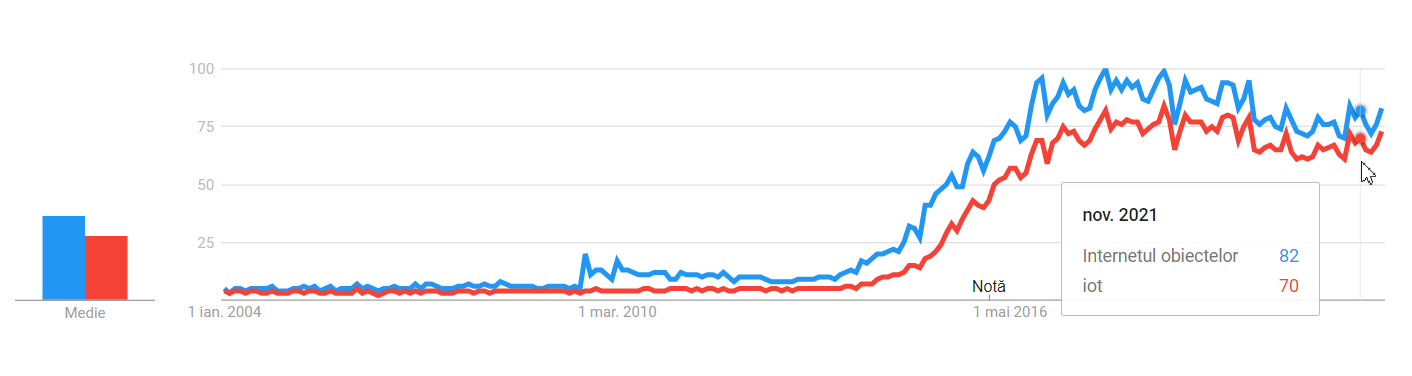
\includegraphics[width=\textwidth]{images/trends_iot.png}
\end{figure}


\section{Structura lucrării}

Capitolul curent a oferit o perspectivă de ansamblu asupra motivației, scopului și temei lucrării. În cele ce urmează, capitolul 2 va prezenta o serie de noțiuni fundamentale pentru înțelegerea subiectelor tratate, oferind definiții și explicații pentru diverse concepte întâlnite în domeniul \acrshort{iot} sau al testării sistemelor informatice. Va fi analizată apoi literatura relevantă temei în vederea conturării obiectivelor lucrării. Capitolul 3 conține o descriere atât teoretică, cât și tehnică a sistemelor \acrshort{iot}, oferind definiții riguroase și exemple de protocoale, arhitecturi și dispozitive utilizate în practică. În capitolul 4 găsim motivația pentru realizarea unui set de aplicații de evaluare pentru tehnicile de testare și descrierea implementării tehnice a unui astfel de \textit{benchmark}. Capitolul 5 continuă prin evaluarea câtorva tehnici de testare pe setul de aplicații propus anterior. Vor fi analizate o serie diversă de tehnici cum ar fi testarea funcțională și de integrare, testarea exploratorie folosind algoritmi de \textit{fuzzing}, analiză statică pentru descoperirea de vulnerabilități în codul sursă, iar în final câteva elemente de analiză cu modelare formală. Concluziile și subiectele ce rămân deschise pentru o cercetare viitoare vor fi expuse în capitolul 6. La finalul lucrării se vor regăsi glosarul termenilor și abrevierilor, bibliografia și anexele conținând cod sursă sau diagrame.